\section{Introduction}

After initialisation, run of the model or computation of diagnostics, 
output Meso-NH files can be convert into other formats of files. 
The present documentation aims at describ the differents tools which can be
applied to the binary part of FM files (their suffix is {\bf .lfi}).
Most of these tools can be run on the user local
computer (Linux PC or HP workstation).
\\

First, the compression tool \texttt{lfiz} and the conversion
tool \texttt{conv2dia} dealing with FM files (synchronous and diachronic)
as input and output, are described. 
The next sections concern tools dealing with other formats than
FM: conversions with \texttt{lfi2cdf}, \texttt{lfi2grb} and \texttt{lfi2v5d}.
A set of tools for reading diachronic FM files and dealing with diachronic 
informations is presented: \texttt{extractdia}, \texttt{mesonh2obs} and 
\texttt{obs2mesonh} (the 2 latest aim at help users to compare MesoNH outputs to
observations).
\\

The figure \ref{fig:fic1} shows when a FM file is either \underline{synchronous}
(contains the values of all the fields corresponding to the same instant of the
simulation) or \underline{diachronic} (contains time series of some fields
obtained during the run of the model). 
Then the figure \ref{fig:toolstab} resumes the tools which can be applied to a
FM file according its type, one of the two previous ones. \\

\begin{figure}[htb]
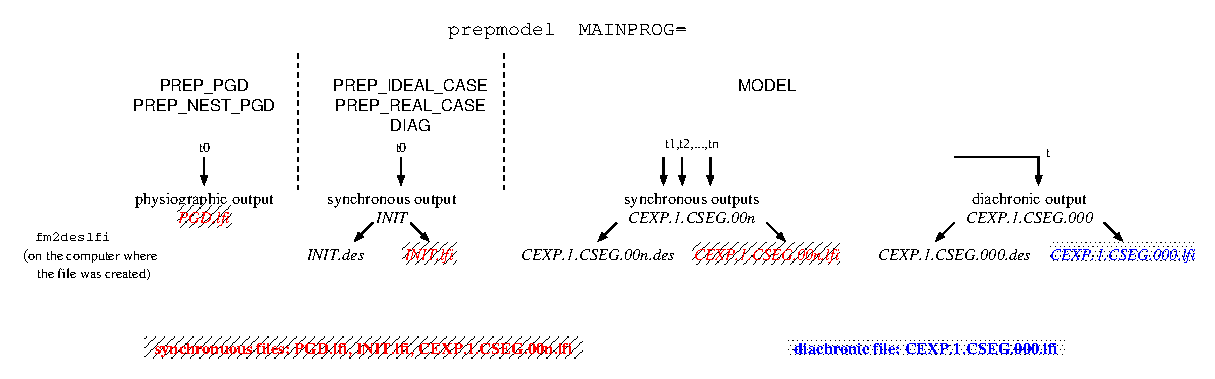
\psfig{file=fic1.eps,width=17cm} 
\caption{Type of FM files after a MesoNH program\label{fig:fic1}}
\end{figure}

\begin{figure}[htb]
\centerline{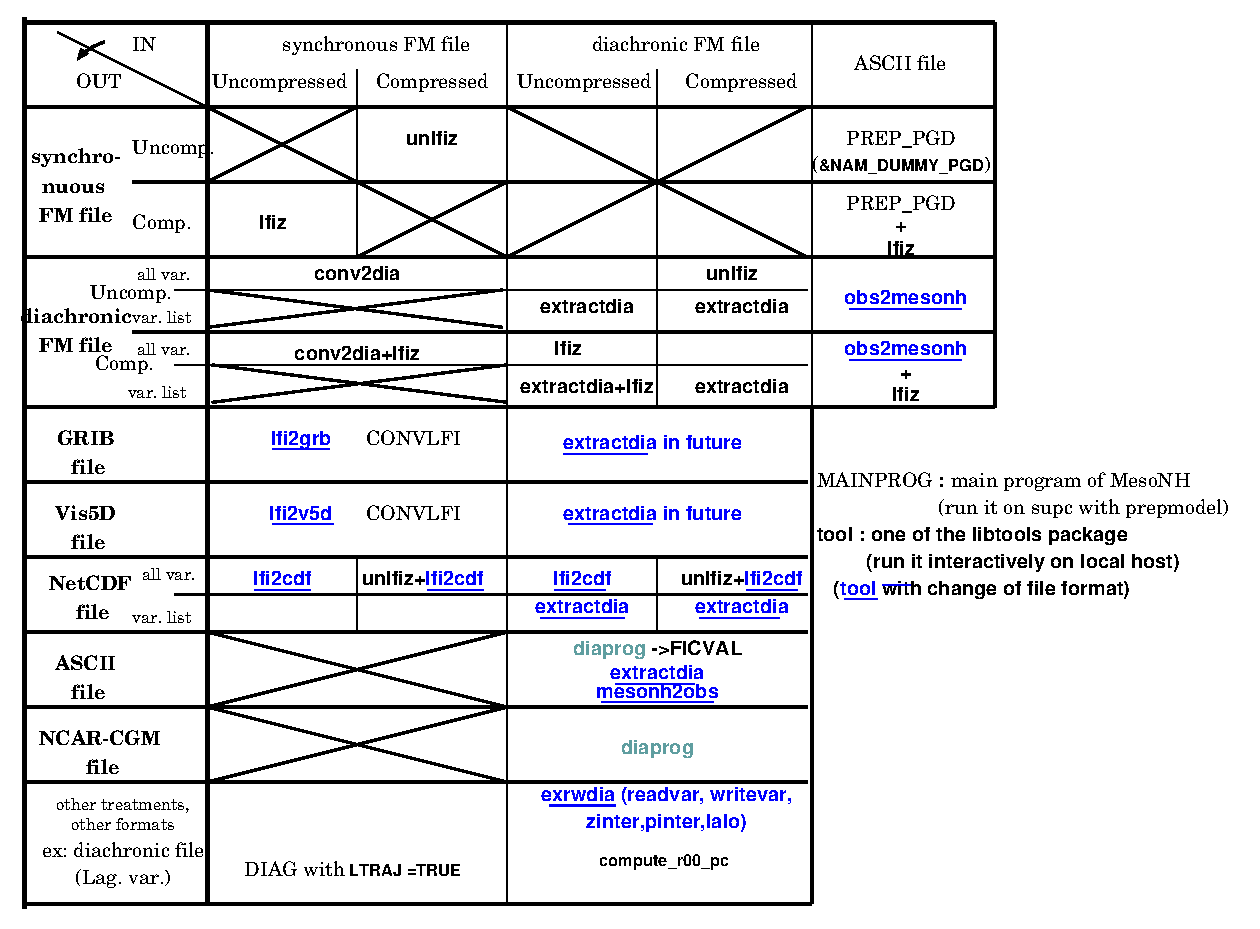
\psfig{file=toolstab.eps,width=17cm} }
\caption{Which tools on FM files? \label{fig:toolstab}}
\end{figure}

